%!TeX root=../pridetop.tex
\chapter[Chapter \thechapter]{}
\begin{figure}[t!]
\centering
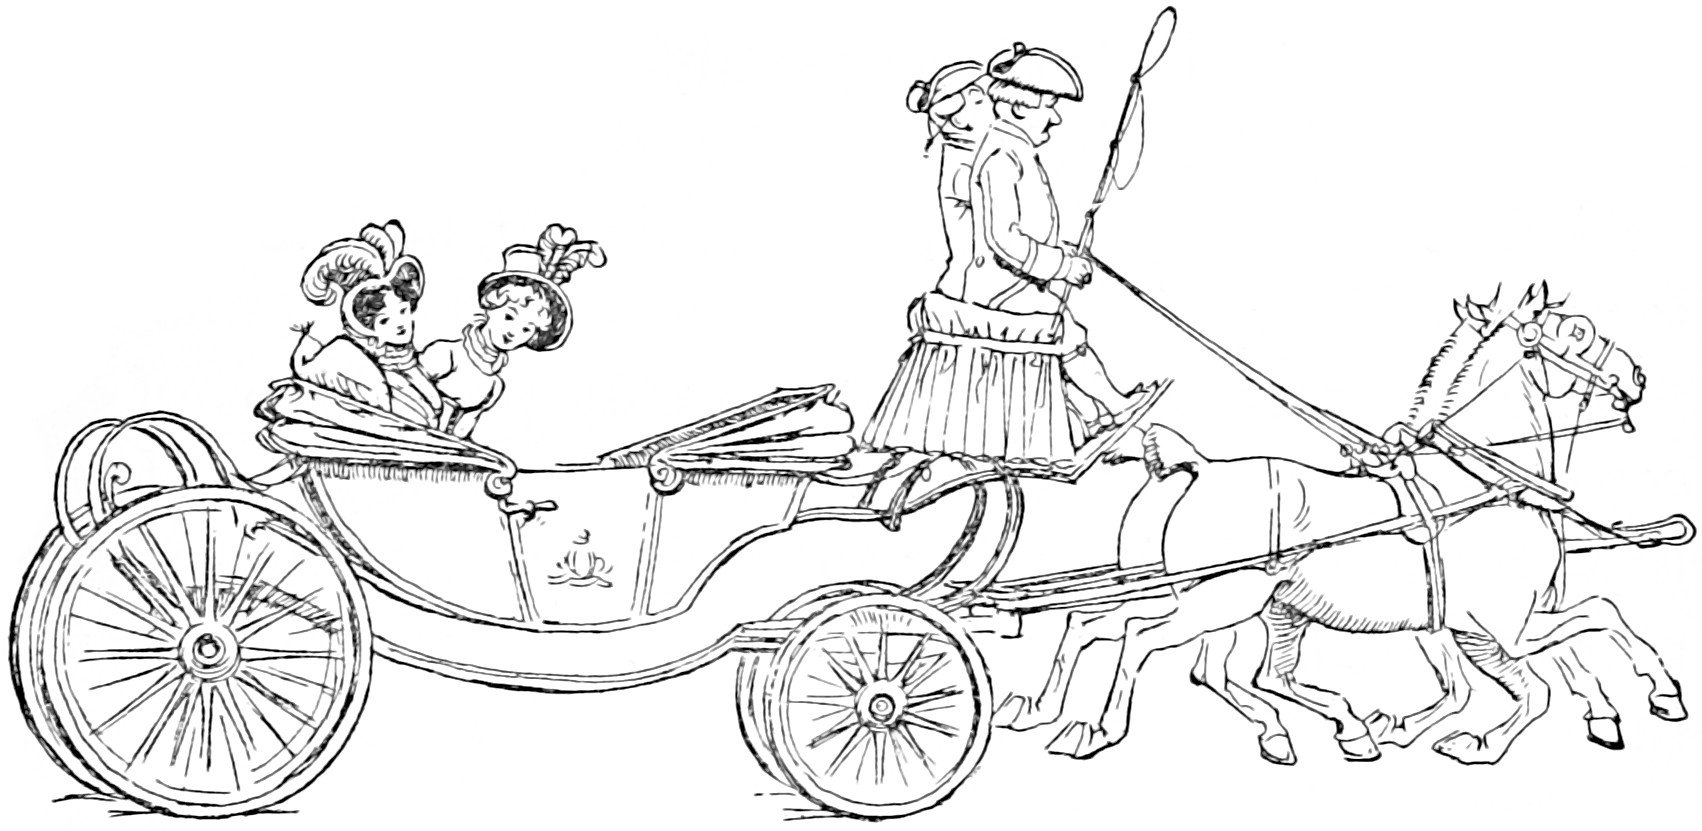
\includegraphics[width=\linewidth]{12top}
\captionlistentry{Headpiece to Chapter \thechapter}
\end{figure}

\vspace{-0.5cm}
\lettrine[lines=8,loversize=.3,image=true]{initials/chap12i}{n}  consequence of an agreement between the sisters, Elizabeth wrote the next morning to her mother, to beg that the carriage might be sent for them in the course of the day. But Mrs Bennet, who had calculated on her daughters remaining at Netherfield till the following Tuesday, which would exactly finish Jane's week, could not bring herself to receive them with pleasure before. Her answer, therefore, was not propitious, at least not to Elizabeth's wishes, for she was impatient to get home. Mrs Bennet sent them word that they could not possibly have the carriage before Tuesday; and in her postscript it was added, that if Mr Bingley and his sister pressed them to stay longer, she could spare them very well. Against staying longer, however, Elizabeth was positively resolved—nor did she much expect it would be asked; and fearful, on the contrary, of being considered as intruding themselves needlessly long, she urged Jane to borrow Mr Bingley's carriage immediately, and at length it was settled that their original design of leaving Netherfield that morning should be mentioned, and the request made.

The communication excited many professions of concern; and enough was said of wishing them to stay at least till the following day to work on Jane; and till the morrow their going was deferred. Miss Bingley was then sorry that she had proposed the delay; for her jealousy and dislike of one sister much exceeded her affection for the other.

The master of the house heard with real sorrow that they were to go so soon, and repeatedly tried to persuade Miss Bennet that it would not be safe for her—that she was not enough recovered; but Jane was firm where she felt herself to be right.

To Mr Darcy it was welcome intelligence: Elizabeth had been at Netherfield long enough. She attracted him more than he liked; and Miss Bingley was uncivil to \textit{her} and more teasing than usual to himself. He wisely resolved to be particularly careful that no sign of admiration should \textit{now} escape him—nothing that could elevate her with the hope of influencing his felicity; sensible that, if such an idea had been suggested, his behaviour during the last day must have material weight in confirming or crushing it. Steady to his purpose, he scarcely spoke ten words to her through the whole of Saturday: and though they were at one time left by themselves for half an hour, he adhered most conscientiously to his book, and would not even look at her.

On Sunday, after morning service, the separation, so agreeable to almost all, took place. Miss Bingley's civility to Elizabeth increased at last very rapidly, as well as her affection for Jane; and when they parted, after assuring the latter of the pleasure it would always give her to see her either at Longbourn or Netherfield, and embracing her most tenderly, she even shook hands with the former. Elizabeth took leave of the whole party in the liveliest spirits.

They were not welcomed home very cordially by their mother. Mrs Bennet wondered at their coming, and thought them very wrong to give so much trouble, and was sure Jane would have caught cold again. But their father, though very laconic in his expressions of pleasure, was really glad to see them; he had felt their importance in the family circle. The evening conversation, when they were all assembled, had lost much of its animation, and almost all its sense, by the absence of Jane and Elizabeth.

They found Mary, as usual, deep in the study of thorough bass and human nature; and had some new extracts to admire and some new observations of threadbare morality to listen to. Catherine and Lydia had information for them of a different sort. Much had been done, and much had been said in the regiment since the preceding Wednesday; several of the officers had dined lately with their uncle; a private had been flogged; and it had actually been hinted that Colonel Forster was going to be married.